\subsection{Komunikasi Servo Kaki}
\begin{figure}[H]
  \centering
  \begin{subfigure}{0.45\textwidth}
    \centering
    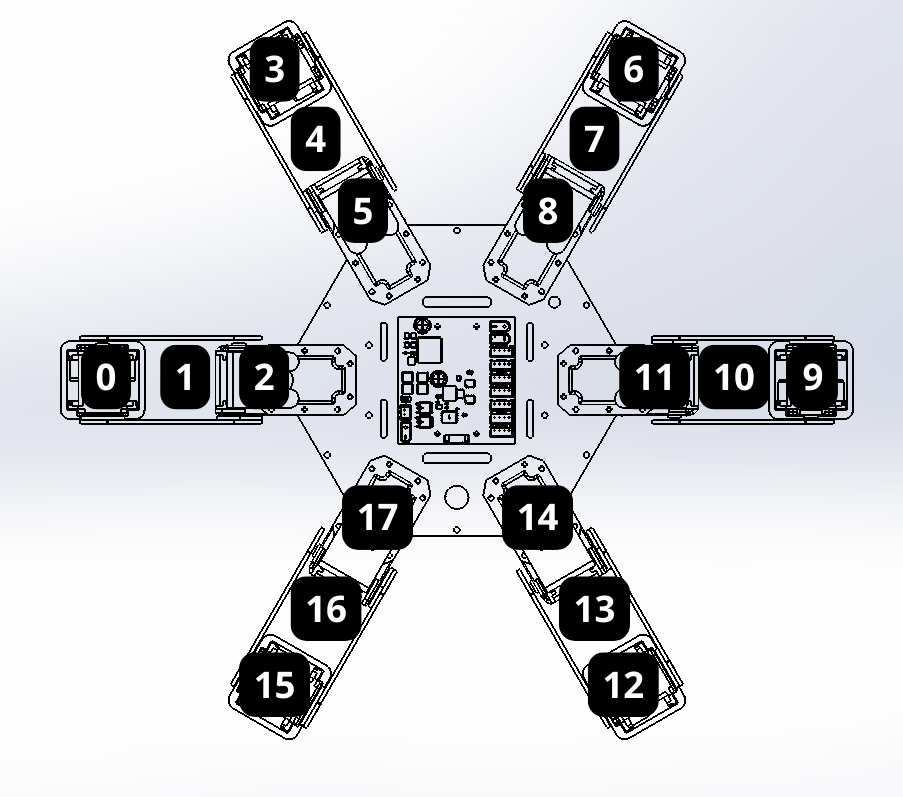
\includegraphics[width=\textwidth]{gambar/ID_Atas.png}
    \caption{Tampak Atas}
    \label{fig:ID_Atas}
  \end{subfigure}
  \hfill
  \begin{subfigure}{0.45\textwidth}
    \centering
    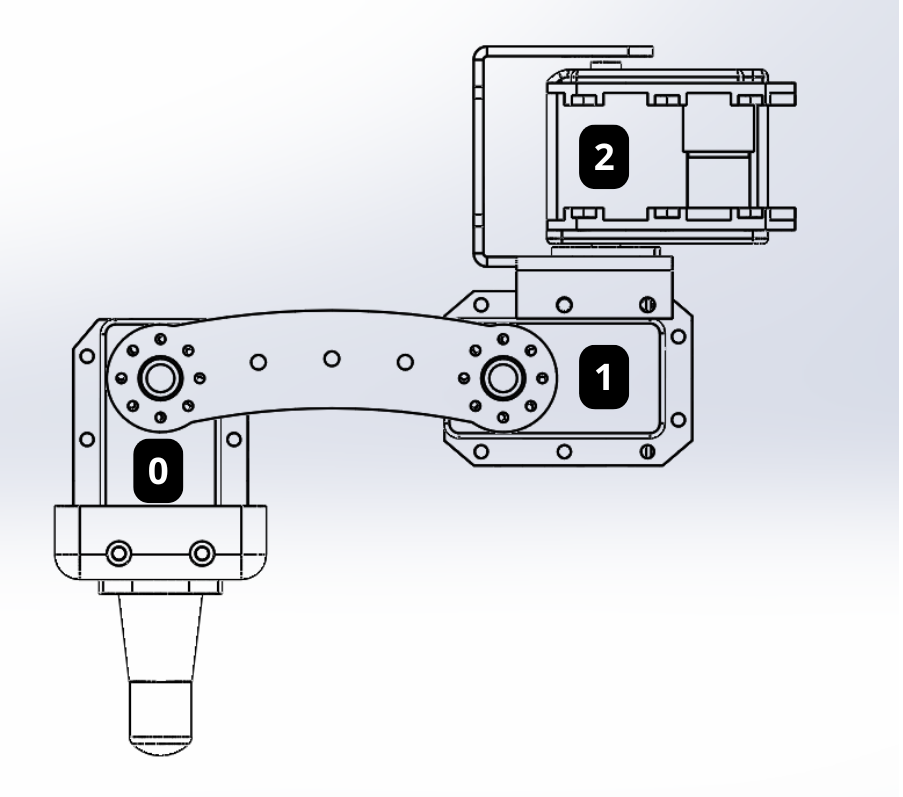
\includegraphics[width=\textwidth]{gambar/ID_Samping.png}
    \caption{Tampak Samping Pada Kaki Pertama}
    \label{fig:ID_Samping}
  \end{subfigure}
  \caption{Penomoran ID Servo Kaki}
  \label{fig:Penomoran_ID}
\end{figure}
Komunikasi antara STM32 dan servo pada kaki robot dimulai dengan menentukan ID
pada setiap servo. Setiap kaki memiliki 3 buah servo. Penomoroan ID servo pada
kaki dimulai dari 0 hingga 17. Terdapat dua jenis servo yang digunakan pada kaki
robot, yaitu \emph{MX-28} dan \emph{RX-28}. Servo \emph{RX-28} digunakan pada 
bagian \emph{coxa} kaki, sedangkan servo \emph{MX-28} digunakan pada bagian \emph{femur} 
dan \emph{tibia}.

Besaran yang dikendalikan pada servo oleh STM32 meliputi posisi dan
kecepatan, sehingga data yang dikirimkan ke servo RX-28 dan MX-28 berupa instruksi untuk
mengatur \emph{goal position} dan \emph{speed}. Untuk meningkatkan efisiensi pengendalian
posisi dan kecepatan servo, digunakan metode \emph{sync write}.

\emph{Sync write} adalah metode komunikasi yang memungkinkan pengendalian beberapa
servo secara bersamaan dengan mengirimkan satu paket data. Dengan menggunakan 
metode ini, STM32 dapat mengirimkan instruksi ke beberapa servo RX-28 dalam satu
paket data, sehingga mengurangi waktu yang dibutuhkan untuk mengirimkan instruksi. 

Format pengiriman data \emph{sync write} adalah sebagai berikut :
\begin{itemize}
  \item Header: 0xFF, 0xFF
  \item Broadcast ID: 0xFE
  \item Lenght: ((L+1)*N)+4, L adalah panjang data dan N adalah jumlah Servo
  \item Parameter1: instruksi \emph{sync write} (0x83)
  \item Parameter2: Alamat data yang akan ditulis
  \item Parameter3: Panjang data yang akan di tulis pada tiap servo
  \item Parameter4: ID servo pertama
  \item Parameter5: Data pertama
  \item Parameter6: Data kedua 
  \item ....
  \item Parameter L+3: Panjang data servo pertama
  \item Parameter L+4: ID servo kedua
  \item Parameter L+5: Data pertama servo kedua
\end{itemize}

Sesuai dengan susunan ID yang sudah ditentukan sebelumnya (0 s.d. 17),
maka pengiriman data dengan metode \emph{sync write} untuk mengendalikan
posisi dan kecepatan servo RX-28 adalah sebagai berikut : 
\begin{itemize}
    \item Data[0] = 0xFF
    \item Data[1] = 0xFF
    \item Data[2] = 0xFE
    \item Data[3] = 5*18 + 4, Panjang data adalah 4 byte dan jumlah servo adalah 18
    \item Data[4] = 0x83
    \item Data[5] = 0x1E, Alamat data yang akan ditulis
    \item Data[6] = 4, 2byte untuk posisi dan 2 byte untuk kecepatan
    \item Data[7] = 0x00, ID servo pertama
    \item Data[8] = \emph{goal position} servo pertama (byte low)
    \item Data[9] = \emph{goal speed} servo pertama (byte high)
    \item Data[10] = \emph{speed} servo pertama (byte low)
    \item Data[11] = \emph{speed} servo pertama (byte high)
    \item  Data[12] = 0x01, ID servo kedua
    \item Data[13] = \emph{goal position} servo kedua (byte low)
    \item Data[14] = \emph{goal speed} servo kedua (byte high)
    \item Data[15] = \emph{speed} servo kedua (byte low)
    \item Data[16] = \emph{speed} servo kedua (byte high)
    \item ....
    \item Data[92] = 0x11, ID servo terakhir
    \item Data[93] = \emph{goal position} servo terakhir (byte low)
    \item Data[94] = \emph{goal speed} servo terakhir (byte high)
    \item Data[95] = \emph{speed} servo terakhir (byte low)
    \item Data[96] = \emph{speed} servo terakhir (byte high)
    \item Data[97] = \emph{checksum}
\end{itemize}
Pengiriman data dari STM32 ke servo dilakukan dengan fungsi \emph{Direct Memory
Access} (DMA) yang diaktifkan pada \emph{USART3}. Fungsi DMA ini digunakan untuk
mengirimkan data dari memori ke \emph{USART} tanpa melibatkan CPU, sehingga
pengiriman data dapat dilakukan secara bersamaan dengan proses lainnya
(\emph{non-blocking}). Baud rate yang digunakan untuk komunikasi adalah
1Mbps, yang mana total waktu yang dibutuhkan untuk mengirimkan satu paket data
adalah (98*8)/1000000 = 0,784 ms.

\subsection{Komunikasi Servo Lengan}
\begin{figure} [H] \centering
    % Nama dari file gambar yang diinputkan
    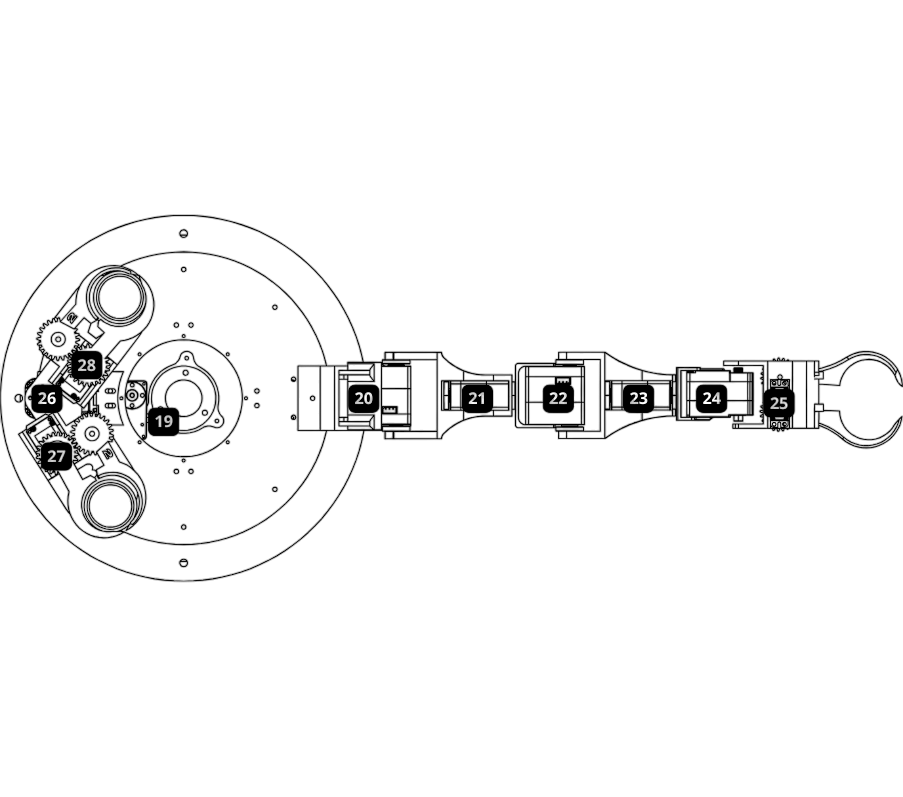
\includegraphics[scale=0.4]{gambar/ID_Kepala.png}
    % Keterangan gambar yang diinputkan
    \caption{Penomoran ID Servo Lengan}
    % Label referensi dari gambar yang diinputkan
    \label{fig:ID_Kepala} 
\end{figure}

Komunikasi antara STM32 dan servo pada kepala dan lengan robot,
sama seperti pada kaki, dimulai dengan menentukan ID pada setiap servo.
Penomoroan ID servo pada kepala dan lengan dimulai dari 19 hingga 25.
Kemudian terdapat 3 buah servo tambahan yang bukan bagian dari lengan. 
Tiga servo ini digunakan sebagai tempat untuk menyimpan objek setelah di 
ambil oleh lengan. Nomor ID yang digunakan adalah 26, 27, dan 28.

Metode komunikasi yang digunakan, sama seperti pada kaki, yaitu \emph{sync
write}. Namun, servo yang digunakan berasal dari manufaktur yang berbeda
(\emph{Feetech}). Hal ini menyebabkan perbedaan alamat data dan jumlah data yang
dikirimkan agar membuat servo berjalan. Jika pada bagian kaki data yang
dikirimkan hanya \emph{goal position} dan \emph{goal speed}, pada servo lengan
data yang dikirimkan terdiri dari \emph{acceleration} (1 byte), \emph{target
position} (2 byte), \emph{target torque} (2 byte), \emph{running speed} (2 byte),
dan \emph{torque limit} (2 byte).

Dengan demikian, pengiriman data ke setiap servo pada bagian kepala robot adalah
sebagai berikut : 
\begin{itemize}
    \item Data[0] = 0xFF
    \item Data[1] = 0xFF
    \item Data[2] = 0xFE
    \item Data[3] = 10*10 + 4, Panjang data adalah 9 byte dan jumlah servo adalah 10
    \item Data[4] = 0x83
    \item Data[5] = 0x29, Alamat data yang akan ditulis
    \item Data[6] = 9, 1byte untuk \emph{acceleration}, 2 byte untuk \emph{target position},
    \emph{target torque}, \emph{running speed}, dan \emph{torque limit}
    \item Data[7] = 0x13, ID servo pertama
    \item Data[8] = \emph{acceleration} servo pertama
    \item Data[9] = \emph{target position} servo pertama (byte low)
    \item Data[10] = \emph{target position} servo pertama (byte high)
    \item Data[11] = \emph{target torque} servo pertama (byte low)
    \item Data[12] = \emph{target torque} servo pertama (byte high)
    \item Data[13] = \emph{running speed} servo pertama (byte low)
    \item Data[14] = \emph{running speed} servo pertama (byte high)
    \item Data[15] = \emph{torque limit} servo pertama (byte low)
    \item Data[16] = \emph{torque limit} servo pertama (byte high)
    \item \dots
    \item Data[97] = 0x1C, ID servo terakhir
    \item Data[98] = \emph{acceleration} servo terakhir
    \item Data[99] = \emph{target position} servo terakhir (byte low)
    \item Data[100] = \emph{target position} servo terakhir (byte high)
    \item Data[101] = \emph{target torque} servo terakhir (byte low)
    \item Data[102] = \emph{target torque} servo terakhir (byte high)
    \item Data[103] = \emph{running speed} servo terakhir (byte low)
    \item Data[104] = \emph{running speed} servo terakhir (byte high)
    \item Data[105] = \emph{torque limit} servo terakhir (byte low)
    \item Data[106] = \emph{torque limit} servo terakhir (byte high)
    \item Data[107] = \emph{checksum}
\end{itemize}

Khusus bagian lengan dan kepala dari robot, setelah melakukan pengiriman data, STM32 akan
meminta servo untuk mengirimkan data posisi dari servo. Hal ini bertujuan 
untuk memastikan bahwa servo telah menerima data yang dikirimkan dengan benar.
Untuk itu, digunakan metode \emph{sync read} yang memungkinkan STM32 untuk
membaca data dari beberapa servo secara bersamaan. Format pengiriman data
\emph{sync read} adalah sebagai berikut :
\begin{itemize}
    \item Header: 0xFF, 0xFF
    \item Broadcast ID: 0xFE
    \item Length: N+4, N adalah jumlah servo
    \item Parameter1: instruksi \emph{sync read} (0x82)
    \item Parameter2: Alamat data yang akan dibaca
    \item Parameter3: Panjang data yang akan dibaca
    \item Parameter4: ID servo pertama
    \item Parameter5: ID servo kedua
    \item \dots
    \item Parameter N+3: ID servo terakhir
    \item Parameter N+4: \emph{checksum}
\end{itemize}

Pada bagian ini, terdapat 2 buah tipe servo yang digunakan, yaitu \emph{STS
series} (untuk ID 19-23) dan \emph{HLS Series} (untuk ID 24-28). \emph{Sync
read} hanya bisa digunakan pada servo yang memiliki tipe yang sama. Oleh karena
itu, pengiriman data \emph{sync read} untuk membaca posisi dari servo akan
dibagi menjadi dua paket data, yaitu untuk servo \emph{STS series} dan \emph{HLS
Series}. Pengiriman data \emph{sync read} untuk servo \emph{STS series} adalah
sebagai berikut :
\begin{itemize}
    \item Data[0] = 0xFF
    \item Data[1] = 0xFF
    \item Data[2] = 0xFE
    \item Data[3] = 9
    \item Data[4] = 0x82
    \item Data[5] = 0x38, Alamat data posisi servo 
    \item Data[6] = 2, Panjang data yang akan dibaca (2 byte)
    \item Data[7] = 0x13, ID servo pertama
    \item Data[8] = 0x14, ID servo kedua
    \item Data[9] = 0x15, ID servo ketiga
    \item Data[10] = 0x16, ID servo keempat
    \item Data[11] = 0x17, ID servo kelima
\end{itemize}
Pengiriman data \emph{sync read} untuk servo \emph{HLS Series} adalah sebagai berikut :
\begin{itemize}
    \item Data[0] = 0xFF
    \item Data[1] = 0xFF
    \item Data[2] = 0xFE
    \item Data[3] = 9
    \item Data[4] = 0x82
    \item Data[5] = 0x38, Alamat data posisi servo 
    \item Data[6] = 2, Panjang data yang akan dibaca (2 byte)
    \item Data[7] = 0x18, ID servo pertama
    \item Data[8] = 0x19, ID servo kedua
    \item Data[9] = 0x1A, ID servo ketiga
    \item Data[10] = 0x1B, ID servo keempat
    \item Data[11] = 0x1C, ID servo kelima
\end{itemize}
Pengiriman data \emph{sync read} ini juga menggunakan fungsi DMA yang diaktifkan
pada \emph{USART2}. Total waktu yang dibutuhkan untuk mengirimkan satu paket data
adalah (12*8)/1000000 = 0,096 ms.

\subsection{Komunikasi Jetson Nano dengan STM32}
\label{subsection: komunikasi_jetson_stm32}
Komunikasi antara Jetson Nano dengan STM32 menggunakan komunikasi USB High Speed
dengan protokol \emph{CDC-ACM} (Communications Device Class - Abstract Control
Model). Protokol ini memungkinkan STM32 untuk berfungsi sebagai perangkat serial
virtual yang dapat diakses oleh Jetson Nano melalui port USB. Pada komunikasi ini,
data dikirimkan dalam bentuk paket data dengan format sebagai berikut :
\begin{itemize}
  \item \emph{Message length} (2 byte)
  \item \emph{data offset} (2 byte)
  \item \emph{sequence number} (1 byte)
  \item \emph{payload} (507 byte)
\end{itemize}
Pengiriman dan penerimaan data semua dilakukan dengan menggunakan fungsi intterrupt
pada USB. Dengan demikian, proses pengiriman dan penerimaan data dapat dilakukan
secara bersamaan dengan proses lainnya (\emph{non-blocking}).

Data yang diterima oleh STM32 dari Jetson Nano berisikan beberapa hal sebagai berikut :
\begin{itemize}
  \item Perintah untuk kaki robot (posisi dan kecepatan servo)
  \item Perintah untuk kepala robot (posisi dan kecepatan servo)
  \item Perintah untuk reset STM32
  \item \emph{timestamp} untuk sinkronisasi waktu
\end{itemize}
Data yang dikirimkan oleh STM32 ke Jetson Nano berisikan :
\begin{itemize}
  \item Teganagan baterai \emph{mainboard} dan \emph{power board}
  \item Status dari servo kaki
  \item Status dari servo lengan dan kepala
  \item Status button
  \item Rate komunikasi 
  \item Total packet loss
  \item Rate byte komunikasi
  \item \emph{timestamp} pada STM32
\end{itemize}

\begin{figure} [H] \centering
    % Nama dari file gambar yang diinputkan
    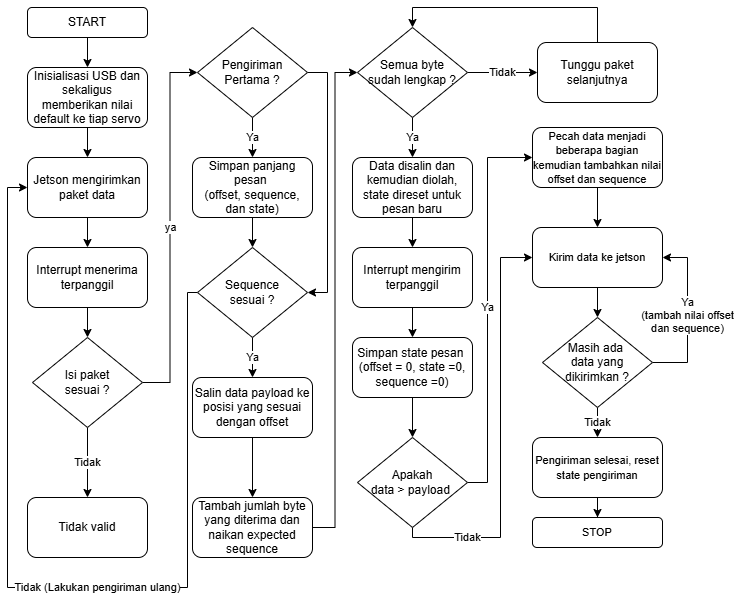
\includegraphics[scale=0.6]{gambar/Komunikasi_USB.drawio.png}
    % Keterangan gambar yang diinputkan
    \caption{Diagram Alir Komunikasi USB}
    % Label referensi dari gambar yang diinputkan
    \label{fig:Komunikasi_USB}
\end{figure}

Proses komunikasi USB ditunjukkan pada Gambar~\ref{fig:Komunikasi_USB}. Pada
sisi penerimaan, setiap kali Jetson Nano mengirimkan paket, interrupt penerimaan
USB dipanggil secara otomatis. Sistem akan memeriksa urutan paket
(\emph{sequence number}), menyusun ulang potongan pesan berdasarkan offset, dan
menggabungkannya menjadi pesan utuh sebelum diolah. Sebaliknya, pada sisi
pengiriman, data yang akan dikirim dipecah menjadi potongan-potongan kecil,
dikirim satu per satu, dan dikontrol melalui interrupt \emph{transmit} hingga
seluruh data terkirim secara utuh. Mekanisme ini menjamin komunikasi berlangsung
tanpa kehilangan urutan paket dan tetap efisien.

Untuk mengelola komunikasi USB dengan STM32, sistem pada Jetson Nano menggunakan
node \emph{communication manager} berbasis arsitektur \emph{publish-subscribe}
dari ROS. Node ini memiliki beberapa \emph{publisher} dan \emph{subscriber} yang
menangani berbagai jenis data seperti perintah gerak kaki, perintah kepala,
status aktuator, pembacaan sensor, serta status tombol. Dengan demikian, node
lain dapat berinteraksi melalui topik ROS tanpa perlu mengetahui detail
implementasi komunikasi USB.

Data hasil komunikasi disimpan dalam \emph{shared memory} yang dilengkapi dengan
mekanisme \emph{mutex} untuk mencegah \emph{race condition} saat data diakses
oleh beberapa proses secara bersamaan. Selain itu, digunakan pula mekanisme
\emph{double buffering} agar pembacaan dan penulisan data dapat berjalan efisien
dan aman.

Sistem komunikasi ini dijalankan secara paralel melalui empat \emph{thread}
menggunakan ROS \emph{multi-threaded spinner}. Masing-masing \emph{thread}
mengeksekusi fungsi callback utama, yaitu:

\begin{itemize}
  \item \emph{usb\_tx\_callback}
  \item \emph{usb\_rx\_callback}
  \item \emph{monitor\_callback}
  \item \emph{legs\_command\_callback}
  \item \emph{head\_command\_callback}
\end{itemize}

Dengan sistem paralel ini, komunikasi Jetson–STM32 dapat berlangsung cepat dan stabil, 
bahkan saat terjadi pertukaran data yang intensif.

\begin{figure}[H]
  \centering
  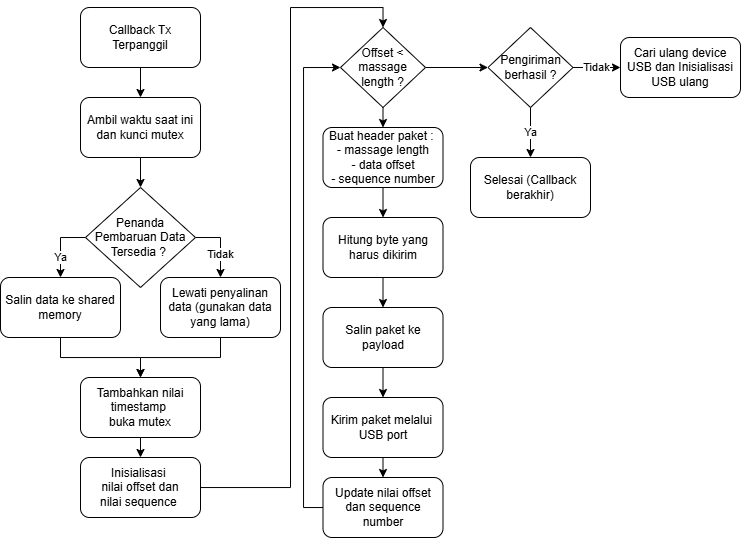
\includegraphics[scale=0.6]{gambar/Jetson_transmit.drawio.png}
  \caption{Diagram Alir Pengiriman Data dari Jetson ke STM32}
  \label{fig:diagram_alir_jetson_transmit}
\end{figure}

Proses pengiriman data ditunjukkan pada Gambar~\ref{fig:diagram_alir_jetson_transmit}. 
Ketika fungsi \emph{usb\_tx\_callback} dipanggil, 
program akan mengunci \emph{mutex} untuk mengakses data yang akan dikirim. 
Setelah memastikan data baru tersedia, 
data disalin ke \emph{shared memory}, 
diubah ke format paket komunikasi sesuai protokol, 
dan dikirimkan ke STM32 melalui USB. 
Bila ukuran data melebihi kapasitas payload, 
data akan dipecah menjadi beberapa paket kecil. 
Jika terjadi kegagalan pengiriman, sistem akan mendeteksi ulang perangkat USB 
dan mencoba mengirim ulang paket.

\begin{figure}[H]
  \centering
  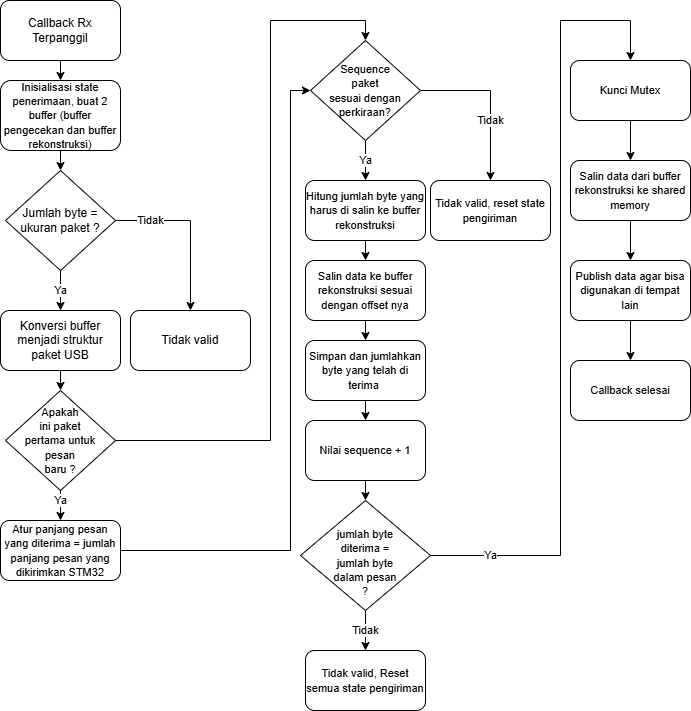
\includegraphics[scale=0.6]{gambar/Jetson_recieve.drawio.png}
  \caption{Diagram Alir Penerimaan Data dari STM32 ke Jetson Nano}
  \label{fig:diagram_alir_jetson_receive}
\end{figure}

Pada Gambar~\ref{fig:diagram_alir_jetson_receive}, 
fungsi \emph{usb\_rx\_callback} bertugas menerima paket data dari STM32, 
memverifikasi ukuran dan urutan paket, 
serta merekonstruksi pesan penuh dari beberapa paket kecil. 
Setelah pesan lengkap diterima, 
data disalin ke \emph{shared memory} dalam keadaan \emph{mutex locked}, 
lalu dipublikasikan ke topik ROS agar dapat diakses modul lain. 
Bila terjadi kesalahan jumlah byte atau urutan paket, 
proses penerimaan akan direset untuk menunggu pesan berikutnya.

Sebelum perintah posisi dan kecepatan dikirim ke mikrokontroler STM32, data
hasil komputasi kinematika pada Jetson Nano yang masih dalam satuan SI (radian
untuk sudut dan rad/s untuk kecepatan sudut) harus dikonversi menjadi nilai
digital yang sesuai dengan karakteristik sinyal servo. Proses konversi ini
dilakukan agar nilai perintah yang dikirim melalui komunikasi serial dapat
langsung dipahami dan dijalankan oleh driver servo di tingkat mikrokontroler.
\begin{equation}
S = \frac{R_{\text{range}}}{\Theta_{\text{range}}} \cdot p
\end{equation}
dengan:
\begin{itemize}
  \item $R_{\text{range}}$ adalah rentang nilai digital yang dapat diterima oleh servo (misalnya 0--4095 untuk resolusi 12-bit),
  \item $\Theta_{\text{range}}$ adalah rentang sudut mekanik servo dalam radian,
  \item $p$ adalah faktor penskalaan tambahan (jika diperlukan untuk kalibrasi atau penyesuaian offset).
\end{itemize}
Dengan demikian, nilai digital posisi servo dihitung menggunakan persamaan:
\begin{equation}
R_{\text{final}} = 
\left[
\left( 
R_{0} + (\theta - \theta_{0}) \cdot 
\frac{R_{\text{range}}}{\Theta_{\text{range}}} \cdot p
\right)
\bmod R_{\text{range}}
\right]_{\text{positif}}
\end{equation}
di mana:
\begin{itemize}
  \item $\theta$ adalah sudut hasil perhitungan kinematika dalam radian,
  \item $\theta_{0}$ adalah sudut referensi (nol mekanik servo),
  \item $R_{0}$ adalah nilai digital yang sesuai dengan $\theta_{0}$,
  \item $\bmod R_{\text{range}}$ memastikan nilai tetap dalam rentang resolusi servo,
  \item operator $_{\text{positif}}$ menjamin hasil akhir bernilai positif.
\end{itemize}
Sedangkan nilai digital untuk kecepatan servo dihitung berdasarkan kecepatan sudut $\omega$ dengan rumus:
\begin{equation}
r = \frac{\omega}{U}, \quad
R = \lfloor r + 0.5 \rfloor, \quad
R_{\text{out}} = \min(R, R_{\max}-1)
\end{equation}
dengan:
\begin{itemize}
  \item $U$ adalah konstanta skala yang mengubah satuan rad/s menjadi satuan digital per satuan waktu servo,
  \item $R_{\max}$ adalah nilai maksimum kecepatan digital yang dapat diterima servo,
  \item operasi pembulatan $\lfloor r + 0.5 \rfloor$ digunakan untuk menghasilkan nilai integer terdekat,
  \item fungsi $\min(\cdot)$ memastikan kecepatan tidak melebihi batas maksimum.
\end{itemize}
Bagian terakhir dari node \emph{communication manager} adalah
\emph{monitor\_callback} yang berfungsi untuk memantau status komunikasi
USB secara berkala. Fungsi ini dijalankan setiap 1 detik untuk menampilkan
bandwidth komunikasi yang sedang berlangsung. Bandwidth komunikasi kemudian
disalin ke \emph{shared memory} agar dapat diakses oleh modul lain dalam sistem.

\subsection{Pembacaan Tegangan Baterai}
Pembacaan tegangan baterai dilakukan dengan menggunakan ADC internal pada STM32.
Terdapat dua buah baterai yang digunakan pada robot, yaitu baterai untuk
\emph{mainboard} dan baterai untuk \emph{driver}. ADC yang digunakan adalah ADC1
pada channel 0 (PA0) untuk membaca tegangan baterai \emph{driver} dan ADC2 pada
channel 11 (PC1) untuk membaca tegangan baterai \emph{mainboard}.

\begin{figure} [H] \centering
    % Nama dari file gambar yang diinputkan
    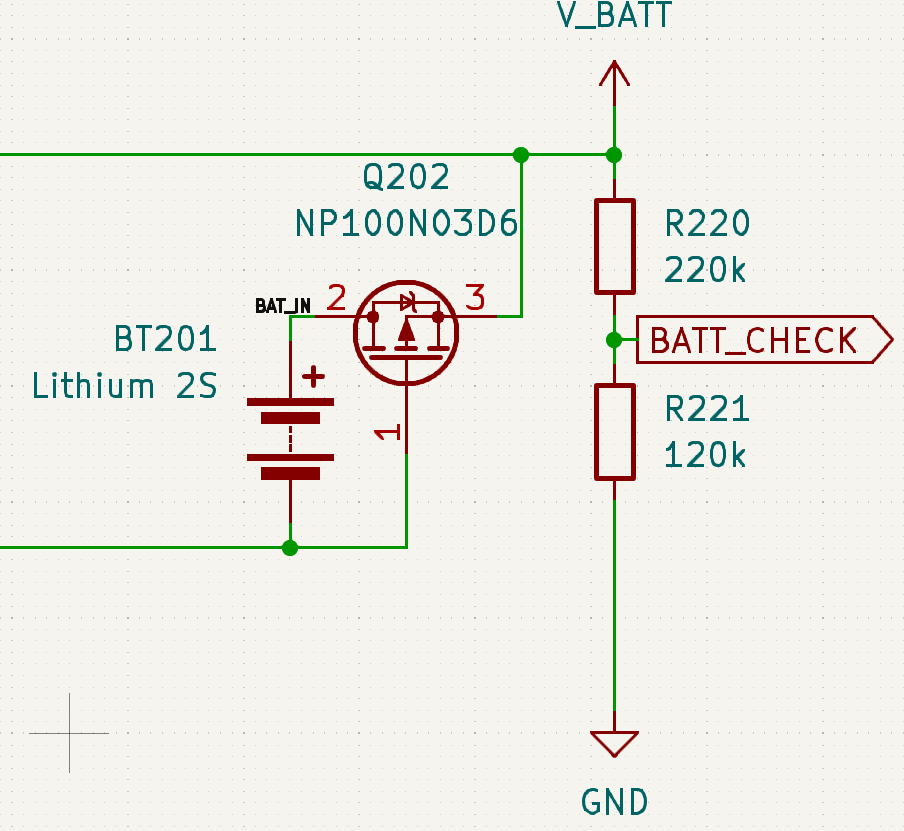
\includegraphics[scale=0.4]{gambar/Batt_check_main_board.png}
    % Keterangan gambar yang diinputkan
    \caption{Pembacaan Tegangan Baterai \emph{Mainboard} dengan ADC}
    % Label referensi dari gambar yang diinputkan
    \label{fig:ADC_Battery}
\end{figure}

Pada STM32, ADC memiliki resolusi 12 bit, sehingga nilai maksimum yang dapat
dihasilkan adalah 4095. Tegangan referensi yang digunakan adalah 3.3V. Untuk 
baterai \emph{driver}, seperti yang sudah dijelaskan pada bagian \ref{sec:driver_board},
tegangan baterai telah di turunkan dengan menggunakan pembagi tegangan dan analog isolator.
Kemudian untuk baterai \emph{mainboard}, tegangan baterai diturunkan dengan menggunakan
pembagi tegangan saja seperti pada gambar \ref{fig:ADC_Battery}. Dengan demikian, rumus untuk menghitung tegangan baterai
adalah sebagai berikut :

\begin{equation}
\begin{aligned}
V_\text{DriverBatt} &=
\frac{\frac{N}{4095}\,V_\text{ref}}
{\frac{R_{18}}{R_{18}+R_{17}}\,\text{Gain}}
= \frac{\frac{N}{4095}\,(3.3)}
{\frac{18}{240+18}\,1.6}
= \frac{\frac{N}{4095}\,(3.3)}{0.1116279}
= \frac{N}{4095}\,\times 29.5625
= N \times 0.00722 \\[1ex]
V_\text{MainBatt} &=
\frac{\frac{N}{4095}\,V_\text{ref}}
{\frac{R_{221}}{R_{221}+R_{220}}}
= \frac{\frac{N}{4095}\,(3.3)}
{\frac{120}{220+120}}
= \frac{\frac{N}{4095}\,(3.3)}{0.352941}
= \frac{N}{4095}\,\times 9.3529
= N \times 0.002285
\end{aligned}
\end{equation}

Pembacaan tegangan baterai dilakukan dengan menggunakan fitur \emph{Direct
Memory Access} (DMA) pada STM32. Fitur ini memungkinkan pembacaan ADC dilakukan
secara \emph{non-blocking}, sehingga pembacaan tegangan baterai dapat dilakukan
bersamaan dengan proses lainnya. Setelah pembacaan selesai, nilai dari ADC
dirata-ratakan dengan menggunakan \emph{exponential moving average} (EMA) untuk
mengurangi noise pada pembacaan. Nilai EMA dihitung dengan rumus berikut :
\begin{equation}
V_\text{out}[n] = V_\text{out}[n-1] + \alpha \bigl( V_\text{in}[n] - V_\text{out}[n-1] \bigr)
\end{equation}

\begin{figure} [H] \centering
    % Nama dari file gambar yang diinputkan
    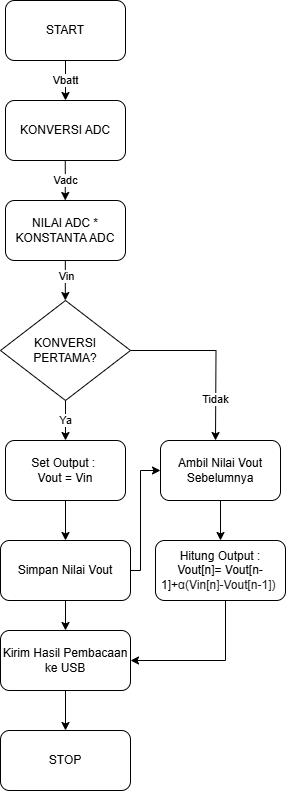
\includegraphics[scale=0.5]{gambar/Pembacaan_Baterai.drawio.png}
    % Keterangan gambar yang diinputkan
    \caption{Diagram Alir Pembacaan Tegangan Baterai}
    % Label referensi dari gambar yang diinputkan
    \label{fig:diagram_alir_baterai} 
\end{figure}

Proses lengkap pembacaan tegangan baterai ditunjukkan pada Gambar 
\ref{fig:diagram_alir_baterai}. Proses dimulai dengan konversi ADC yang berlangsung
secara terus-menerus menggunakan DMA. Setelah konversi selesai, nilai ADC
disimpan dan dikalikan dengan faktor pengali sesuai pembagi tegangan. Apabila
pembacaan tersebut merupakan pembacaan pertama, nilai hasil konversi langsung
disimpan sebagai nilai keluaran dan dikirim ke Jetson Nano. Untuk pembacaan
selanjutnya, nilai ADC dirata-ratakan dengan EMA terlebih dahulu sebelum
dikirimkan ke Jetson Nano. 